\chapter{Software Design}\label{chapter:softwaredesign}

\paragraph{Opening paragraph - a chapter to examine how the model was
  broken down in to smaller software objects to be easier to manage
  (each object has its own, tighter focus. Plus examine the
  requirements and dependencies of this project.}

Chapter \ref{chapter:model} defined the model conceptually. This
chapter will describe the implementation of the model in software. The
implementation has two parts. There is the application code written
specifically for this project and there are the dependencies in the
form of libraries and applications written by others. One aim of this
chapter is to serve as a starting guide to anyone who wished to edit
the code later.


\section{Requirements \& Dependencies}
  \paragraph{Description of what fits in this requirements and
    dependencies chapter}
This section will give a brief description of the third-party
libraries and applications required to run the simulation. The
simulation is a Java application. The application uses the libraries that make up the Repast Simphony
framework. In order to run the simulation it is also necessary for the
application to talk to a MySQL database. Finally some of the unit 
tests make use of the EasyMock mocking library 

  \subsection{Java}
  The ease of installing and getting a simulation running was one of
  the reasons why I chose to use Repast Simphony. It also removed the
  choice of language and code editor since there is an
  installer for my development platform (Mac OS X Lion) that installs a version of the Eclipse IDE
  with the Repast Simphony libraries built-in as well of lots of
  helpful functionality such a pre-setup launchers to run the simulation
  with the required libraries already on the classpath. It used
  version 6.?? of the Java Runtime Environment and version ?? Java Development Kit.

  Repast Simphony does allow agent behaviour to be defined using the
  ReLogo dialect of Logo, a point-and-click flowcharts or
  Groovy. However, as a computing student rather than a social
  scientist with little programming experience I decided that the
  simplicity of a ReLogo or flowchart approach would not be worth the
  amount of control I would have to give up. Therefore I decided to use neat Java so I could gain more
  experience using the Java language and
  access to the full range of libraries available for Java.

  \subsection{Repast Simphony}
  This project uses Repast Simphony version 2.0.1, the most recent
  release at the time of starting. Documentation can be found on the
  Repast Simphony website. This includes installation and getting
  started guides as well as API documentation. Plus the framework is
  open source so it is possible to dive into source code. For this
  report I do not
  expect the reader to have any experience of Repast Simphony and I
  will describe how I made use of
  particular parts of it. However, I will not go into detail about
  their implementation nor discuss Repast Simphony's full set of
  features. The interested reader is free to
  examine the documentation written by Repast's authors.

  \subsubsection{Contexts and ContextBuilder interface}

  \subsubsection{ContinuousSpace}

  \subsubsection{ScheduledMethod annotation}

  \subsubsection{Network interface}

  \subsubsection{siver.rs folder and XML config}



  \subsection{MySQL}
  This project uses MySQL version 5.?.??. The version that was already
  installed. With JDBC it is very easy to connect to databases in
  Java. The only requirements for the project code is access to the
  MySQL JDBC driver at run time, which is readily available from the
  MySQL website. 

  For this project it is assumed that the database server is running locally. Changing
  this is clearly possible but not in the scope of this project.

  The simulation can dynamically connect to different databases on the server. When connecting to the
  database, the application checks the value of the DB\_ENV
  environment variable (defaulting to ``development'' if not set) and then appends that to ``siver\_'' to make the
  name of the database. This is a trick I learnt from Ruby on
  Rails. It means it is safe to develop the application which may result
  in junk data being placed in the ``development'' database. I can then switch to ``production'' mode when the
  time comes to run proper experiments and be sure that
  all the data is ``clean''. Section \ref{software:experiment} will
  cover the expected schema of the database.


  \subsection{EasyMock}
  There are some unit tests to go with the application code. I am a
  firm believer in the advantages of test driven development. I
  believe for an agent-based model they are important for ensuring
  that the simple behaviour of objects and agents is correct so that
  we can be more confident any emergent behaviour while running the
  simulation is an outcome of the model rather than software
  bugs.

  I used EasyMock in order to use mock objects when testing the
  interactions between the more complicated objects in the
  application. As it names suggests, EasyMock was easy to integrate
  into the project (making the EasyMock libraries and its dependencies
  available at run time). However, since this is not a software
  engineering project, there will be no more detail on the tests. In
  fact, EasyMock itself can be ignored by anyone not wishing to run
  the unit tests.

\section{Application Overview}
This section will give a brief overview of the packages that make up
the application. The following sections then look at each of the
packages in more detail. 

The River, Boat and Cox packages map
naturally to the 3 main types of objects in the model (with the
Boathouse contained in the River package). The model was
then broken down into smaller software classes within these packages. This
makes the software easier to manage as each class has a smaller focus
compared to the larger objects in the model.

The pseudo-UML Figure \ref{software:fig:modeloverview} used before in Chapter \ref{chapter:model} is also a
good starting point for seeing how the main packages relate to each
other. There are some extra entities in the software version. There
is the Experiment package.

\begin{figure}
\begin{center}
  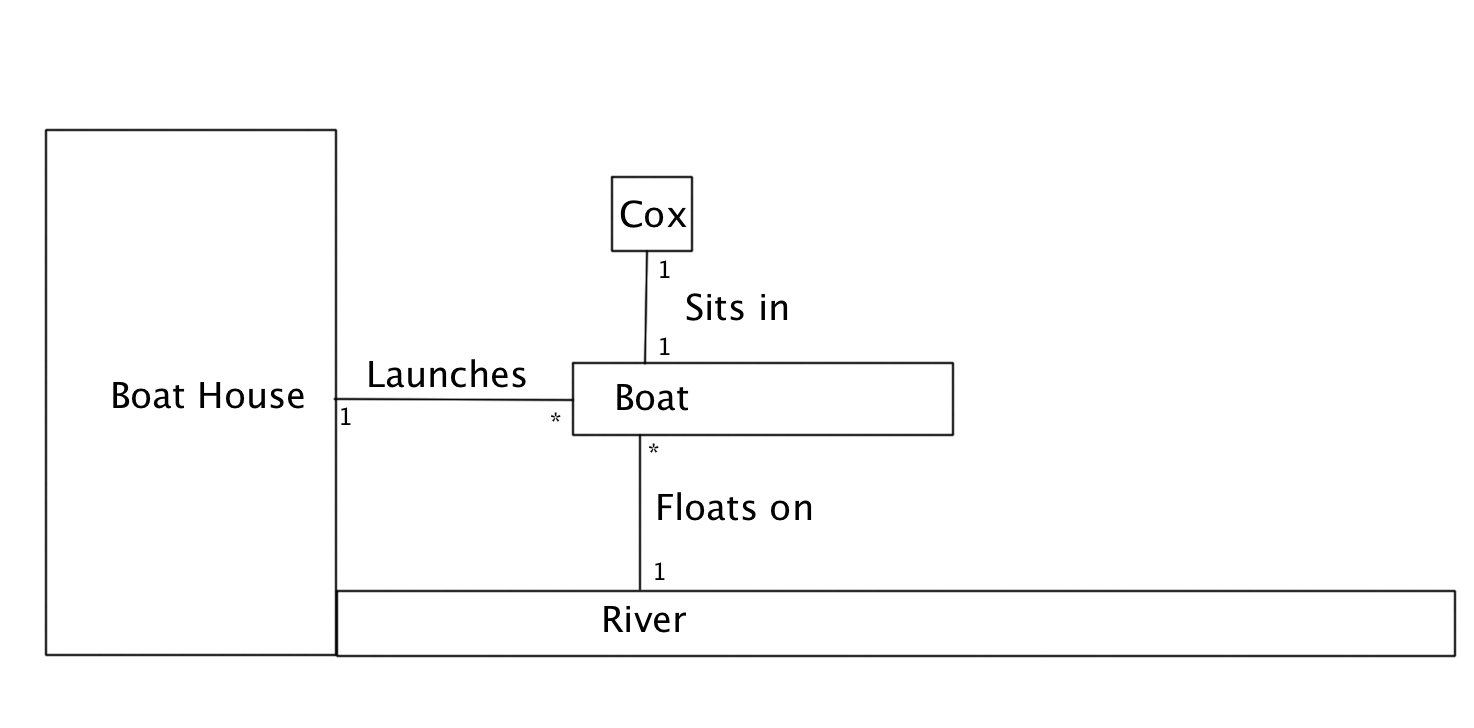
\includegraphics[scale=0.3]{images/ModelOverview.png}
  \caption{Model Overview}
  \label{software:fig:modeloverview}
\end{center}
\end{figure}



\section{River package}
\paragraph{Opening paragraph and UML diagram}
\subsection{River class}

\subsection{Lane class}

\subsection{LaneNode class}

\subsection{LaneEdge class}

\subsection{LaneChangeEdge and TemporaryNode classes}

\subsection{Boathouse class}

\subsection{RiverFactory class}

\subsection{Crash class}


\section{Boat package}
\paragraph{Opening paragraph and UML diagram}
\subsection{Boat class}

\subsection{BoatNavigation class}
      \paragraph{Keeping track of things like current edge and directions of travel (upstream or downstream)}
      \paragraph{Keeping in sync location of cox and boat in 2D space and on the 1D lane graph}

\section{Cox package}
\paragraph{Opening paragraph}

\subsection{Cox class}
\paragraph{scheduling decision making}
\subsection{CoxObservations class}
\paragraph{how observations are made available to cox brain}
\subsection{CoxBrains}

\subsection{Actions}

    \paragraph{executution}
    \paragraph{handling }
    \paragraph{inheritance of different actions}

\section{Experiment package}\label{software:experiment}
\paragraph{Opening paragraph}

\subsection{Database schema}
\paragraph{ER diagram}


\section{Style and UI packages}
\paragraph{Opening paragraph - boat, river and boathouse as displayed
  objects in visualization, UI class for demoing/testing purposes}


\paragraph{Chapter Closing paragraph}
